\chapter[Results]{Results}


This chapter presents the outcomes obtained from the development and implementation of the web-based platform for visualizing air quality forecasts. The platform prototype enables users to interactively explore forecasts of atmospheric pollutants provided by the Copernicus Atmosphere Monitoring Service (CAMS), offering both spatial and temporal insights. In this chapter, the functionality and performance of the platform are analyzed, highlighting key features such as dynamic map layers, point-specific pollutant queries, time-series visualizations, forecast animations, and data export capabilities. Each section illustrates how the interface supports intuitive exploration of forecast data and facilitates interpretation of pollutant concentrations across different geographic domains and forecast horizons.

\section{Main Interface}

The application runs entirely in the web browser, so it does not require installation or additional configuration. 
Its central element is an interactive map, implemented with \texttt{Leaflet}, which displays pollutant concentration layers provided by CAMS through the WMS standard. 
Users can select both the geographic domain (Europe or Global) and the pollutant of interest through a drop-down menu. 
A time slider positioned below the map allows exploration of hourly forecasts up to four days ahead, while an adaptive legend facilitates interpretation of concentration values by associating each color range with a quantitative interval (Figure~\ref{fig:interface-extra}).

In addition to these basic elements, the platform includes complementary features designed to enhance usability and interactivity. 
The map itself is fully interactive: by clicking on any location, the application retrieves the forecasted pollutant value at that point and displays it in a dedicated text panel and also it will display the future values in the time-series plots. 
Animation controls enable sequential visualization of forecasts, helping users to perceive the temporal evolution of pollutant dispersion. 
These elements are illustrated in Figure~\ref{fig:interface}, which highlights the pollutant and time indicators, the clickable map for pollutant extraction, and the animation controls.
Furthermore, the interface integrates a charting component that generates time-series plots of pollutant concentrations at the selected location, together with export options that allow downloading the data for further analysis (Figure~\ref{fig:interface-extra}).

\begin{figure}[h]
	\centering
	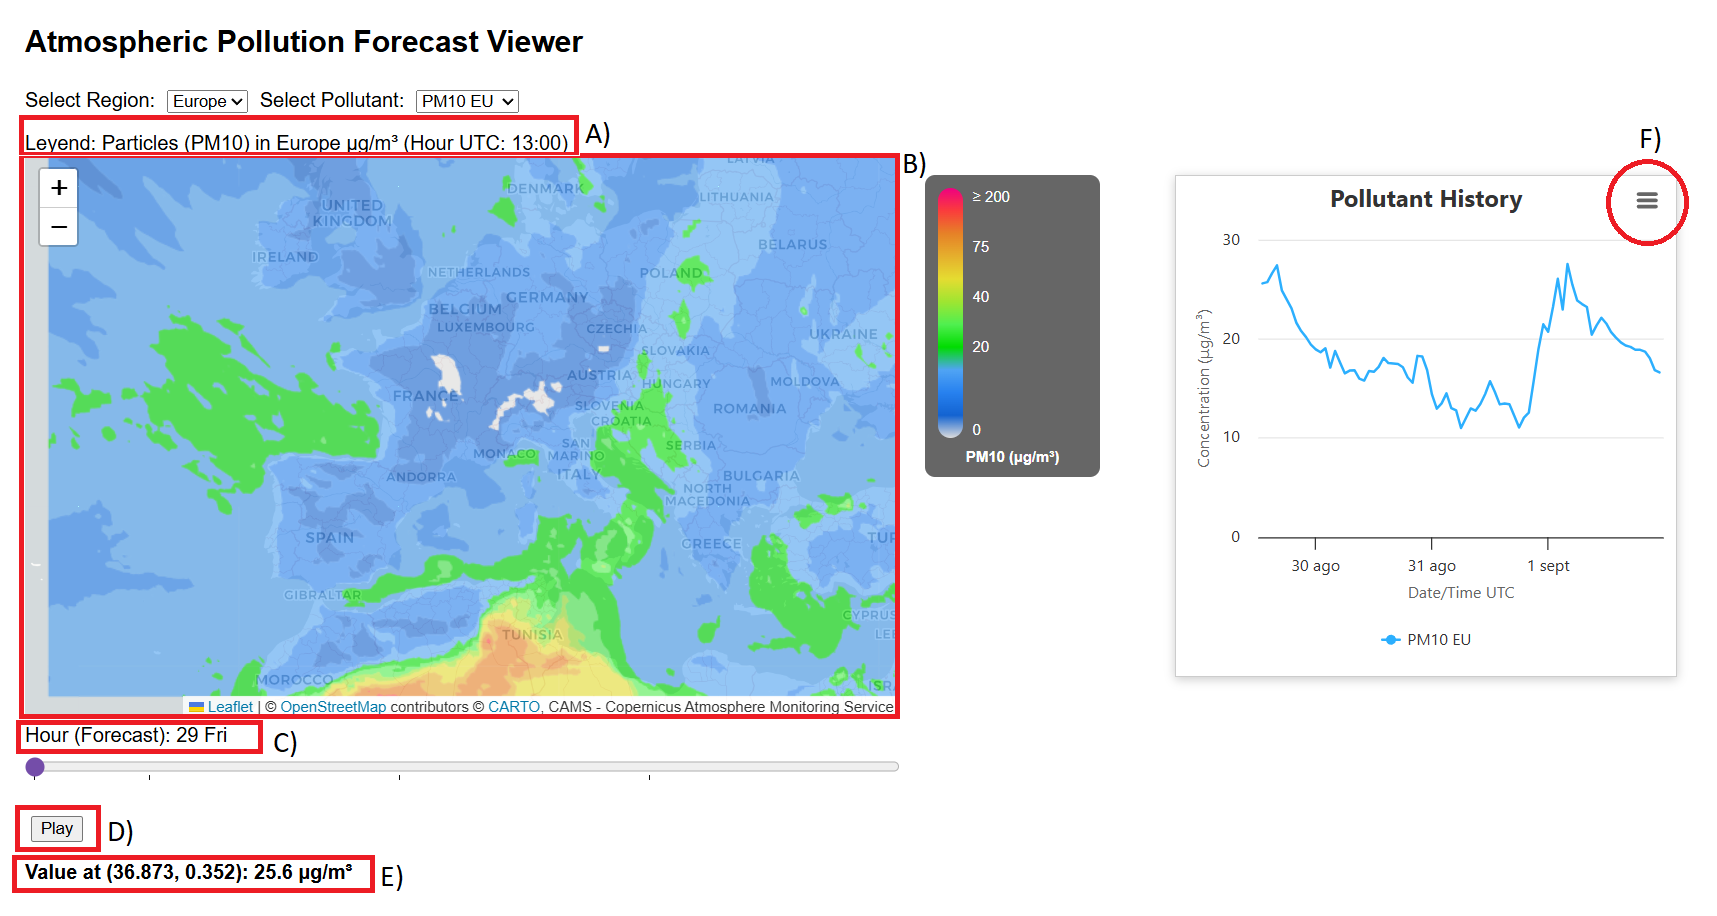
\includegraphics[width=0.9\textwidth]{fig/resultados-interfaz-mapa.PNG}
	\caption{Main user interface of the developed platform.
		(A) Text panel indicating the selected pollutant and forecast hour. 
		(B) Interactive map with clickable locations for pollutant value extraction. 
		(C) Text panel showing the selected forecast day.  
		(D) Animation controls for sequential forecast visualization.
		(E) Text panel displaying the clicked location and its pollutant value.  
		(F) Menu for data download options from the chart.}
	\label{fig:interface}
\end{figure}

\begin{figure}[h]
	\centering
	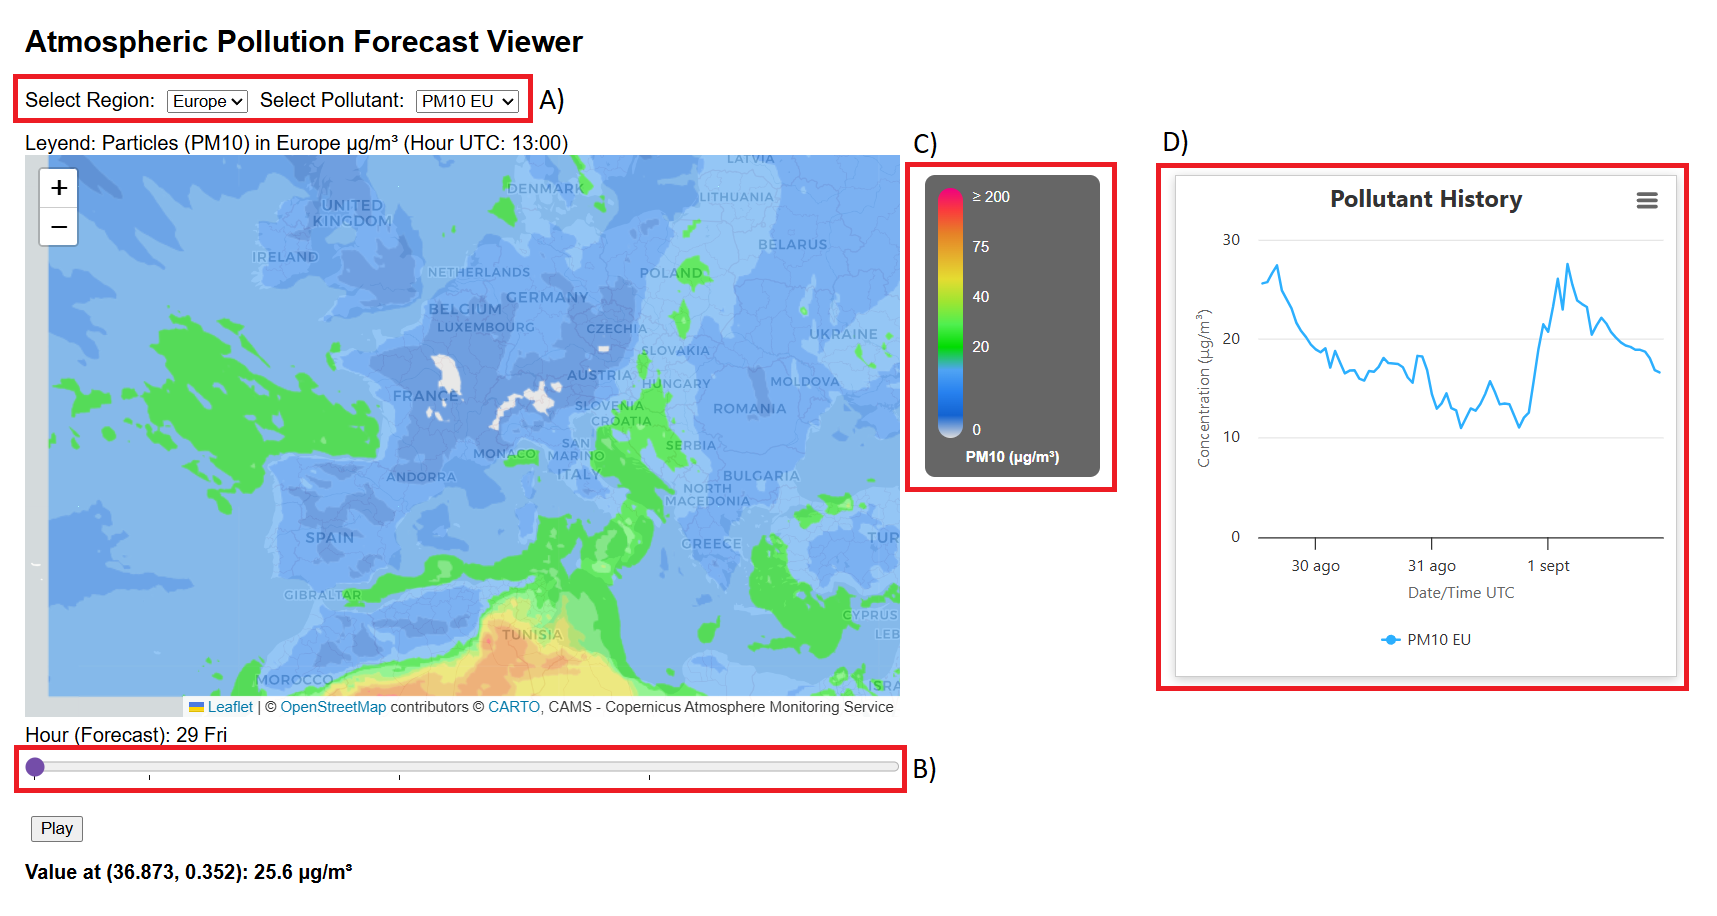
\includegraphics[width=0.9\textwidth]{fig/resultados-interfaz-editada.PNG}
	\caption{Extended view of the platform interface. 
		(A) Region and pollutant selectors.
		(B) Time slider for navigating forecast hours. 
		(C) Color scale legend indicating pollutant concentration levels.
		(D) Time-series chart showing the evolution of pollutant concentrations (example: PM\textsubscript{10}) at the selected location.}
	\label{fig:interface-extra}
\end{figure}


\section{Dynamic Layer Updating}
One of the key features of the platform is the automatic update of pollutant layers whenever the user modifies any of the control parameters: selected region, pollutant, or forecast hour. The update process is triggered first through the region and pollutant selectors  (A) in Figure~\ref{fig:interface-extra}, implemented as dropdown menus, which allow switching between the European or Global domain and choosing the pollutant of interest. Similarly, the time slider (B) in Figure~\ref{fig:interface-extra} enables navigation across the hourly forecasts, and each movement of the slider synchronizes the map with the concentration values corresponding to the selected forecast hour. Finally, the clickable map interaction (B) in Figure~\ref{fig:interface} provides pollutant concentration values for any chosen location. When a location is clicked, the application retrieves the forecasted value for that point, displays it in the corresponding text panel, and simultaneously generates its temporal evolution in the time-series chart (D) in Figure~\ref{fig:interface-extra}. In this way, the interface ensures that all visual elements remain consistent with user selections, offering a smooth and responsive exploration of the CAMS forecast data.



\section{Point Query of Concentrations}
In addition to the dynamic update of pollutant layers, the platform allows users to query
the concentration value at any geographic location by simply clicking on the map. This
interaction triggers a \texttt{WMS GetFeatureInfo} request to the CAMS server, which
returns the forecasted concentration for the selected pollutant and time. 

Once retrieved, the raw value is automatically converted into standardized units
(typically $\mu g/m^3$) through predefined conversion factors that account for the different
formats used by CAMS layers. The resulting value is then displayed in the information
panel (E) in Figure~\ref{fig:interface}, alongside the geographic coordinates of the clicked
location. 

However, when the selected domain is restricted to Europe, the system also validates
whether the clicked location lies inside the spatial coverage of the European forecast. 
If the query is made outside this domain, the application informs the user that the value is
not available for that point. As an illustrative example, Figure~\ref{fig:point-query} shows
the result of clicking on a location outside the European forecast area, where the
information panel explicitly indicates that the data are unavailable. 

This functionality provides users not only with direct access to numerical values within the
forecast domain, but also with clear feedback when attempting to query outside the valid
region, thereby improving transparency and user experience.


\begin{figure}[h]
	\centering
	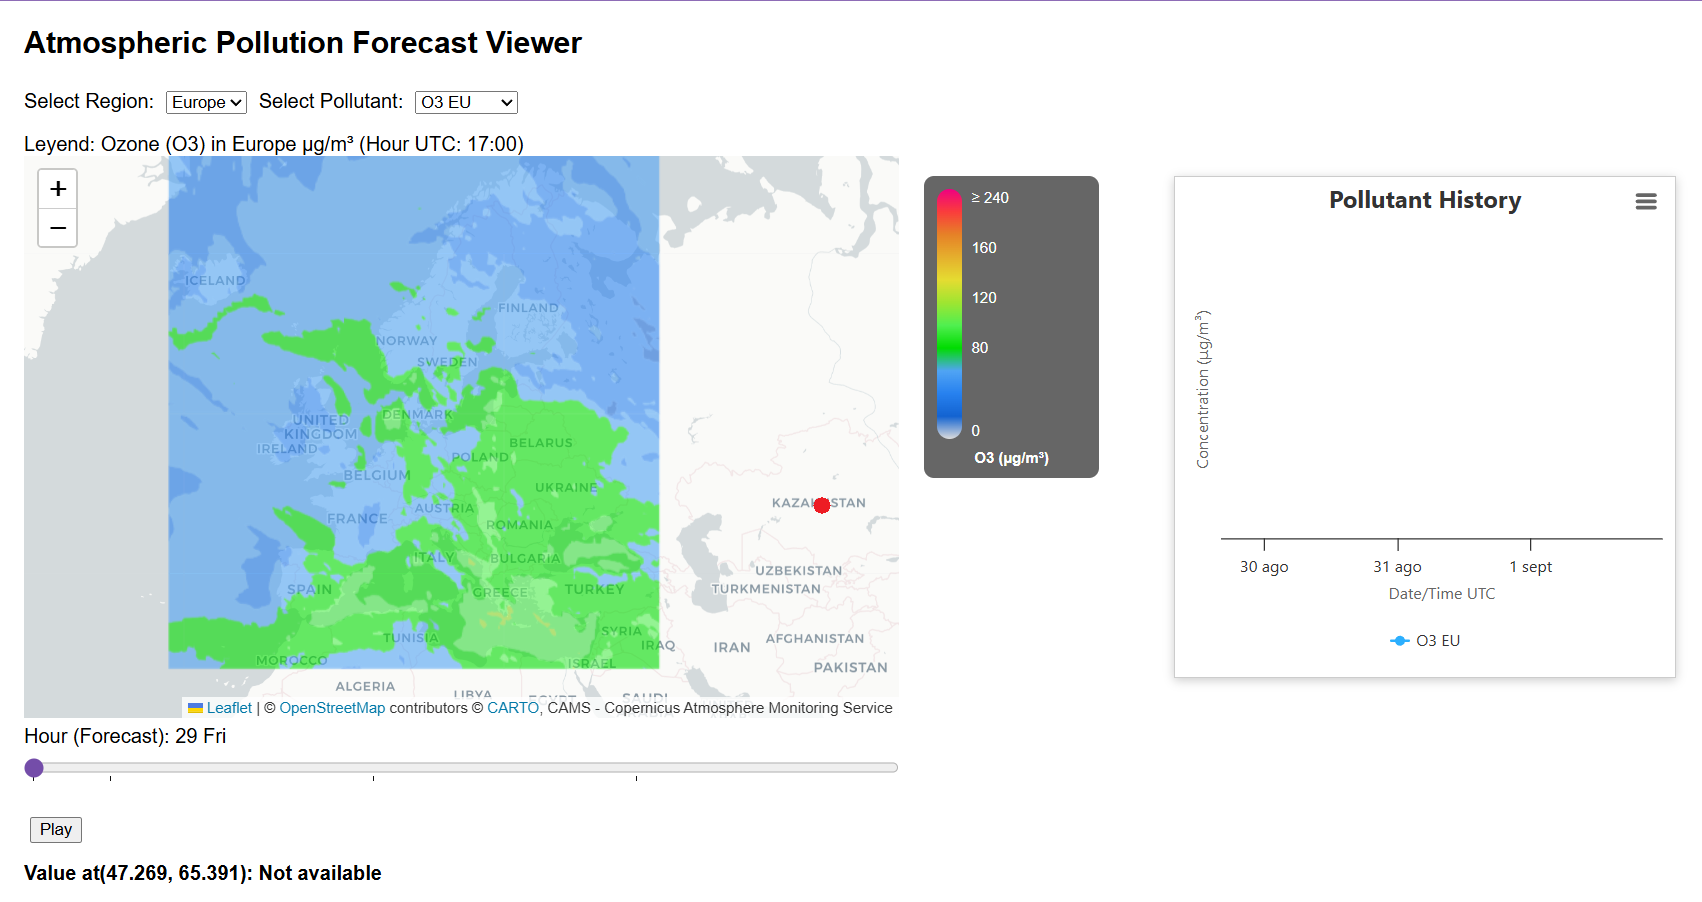
\includegraphics[width=0.9\textwidth]{fig/outofrange.PNG}
	\caption{Example of point query outside the European forecast domain. 
		The red point indicates the clicked location beyond the coverage area, and the information panel shows that the value is not available.}
	
	\label{fig:point-query}
\end{figure}


\section{Time Series Visualization}

The time-series visualization module provides users with an overview of the temporal evolution of pollutant concentrations at any selected location. Once a point is clicked on the interactive map, the platform automatically generates a chart showing the pollutant values for successive forecast hours. Users can also export the data displayed in the chart as a CSV or XLS file for further analysis. This feature facilitates offline processing, statistical analysis, or integration with other tools.

A key aspect of the CAMS forecasts is their temporal resolution, which differs between domains. The European domain delivers predictions at 1-hour intervals, so the concentration values in the chart change every hour, as illustrated in Figure~\ref{fig:timeseries-europe}. In contrast, the Global domain provides predictions at 3-hour intervals, causing the values to remain constant over each 3-hour block before updating at the next forecast step, as shown in Figure~\ref{fig:timeseries-global}. This difference reflects the underlying temporal resolution of the numerical models and should be considered when interpreting pollutant trends.

\begin{figure}[h]
	\centering
	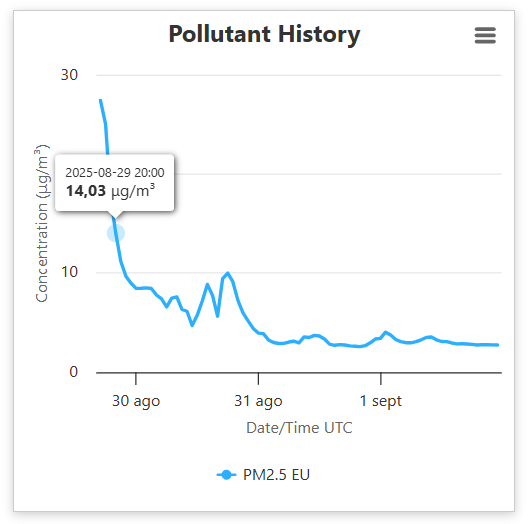
\includegraphics[width=0.25\textwidth]{fig/timeseries-europe.PNG}
	\caption{Time-series visualization of PM\textsubscript{2.5} concentrations at a selected location within the European domain. Values update every hour according to the temporal resolution of the forecasts.}
	\label{fig:timeseries-europe}
\end{figure}

\begin{figure}[h]
	\centering
	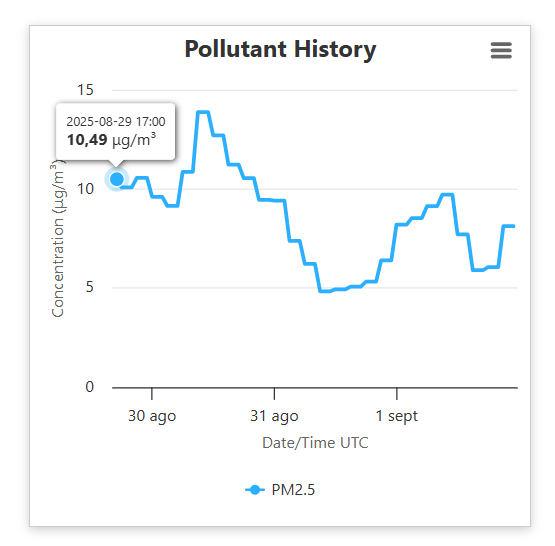
\includegraphics[width=0.25\textwidth]{fig/timeseries-global.PNG}
	\caption{Time-series visualization of PM\textsubscript{2.5} concentrations at a selected location within the Global domain. Values remain constant over 3-hour intervals, corresponding to the temporal resolution of the CAMS forecasts.}
	\label{fig:timeseries-global}
\end{figure}


\subsection{Data Export}

In addition to the time-series visualization, the platform allows users to export the pollutant data for further analysis. The chart interface provides a download button that lets users save the data in CSV or XLS format. This feature enables offline processing, statistical evaluation, or integration with other software tools.

Figure~\ref{fig:data-export} shows an example of the export button in the chart interface and a sample of the downloaded CSV file.

\begin{figure}[h]
	\centering
	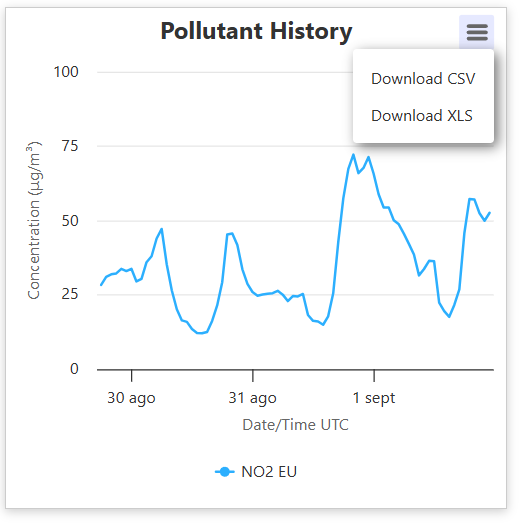
\includegraphics[width=0.25\textwidth]{fig/data-export.png}
	\caption{Export functionality for pollutant time-series data. Users can download the values displayed in the chart for further analysis.}
	\label{fig:data-export}
\end{figure}



\section{Forecast Animation}
To further enhance the understanding of temporal pollutant dynamics, the platform includes a forecast animation feature. By activating the play button, the application sequentially advances the time slider, updating the pollutant layer on the map and the associated legend in real time. This animation allows users to intuitively perceive the spread and evolution of pollutants over the selected domain without manually moving the slider.
For illustration purposes, the UV Index was chosen as an example, since its changes are clearly visible as the slider moves (see Figure~\ref{fig:forecast-animation}).


\begin{figure}[h!]
	\centering
	\begin{subfigure}[b]{0.23\textwidth}
		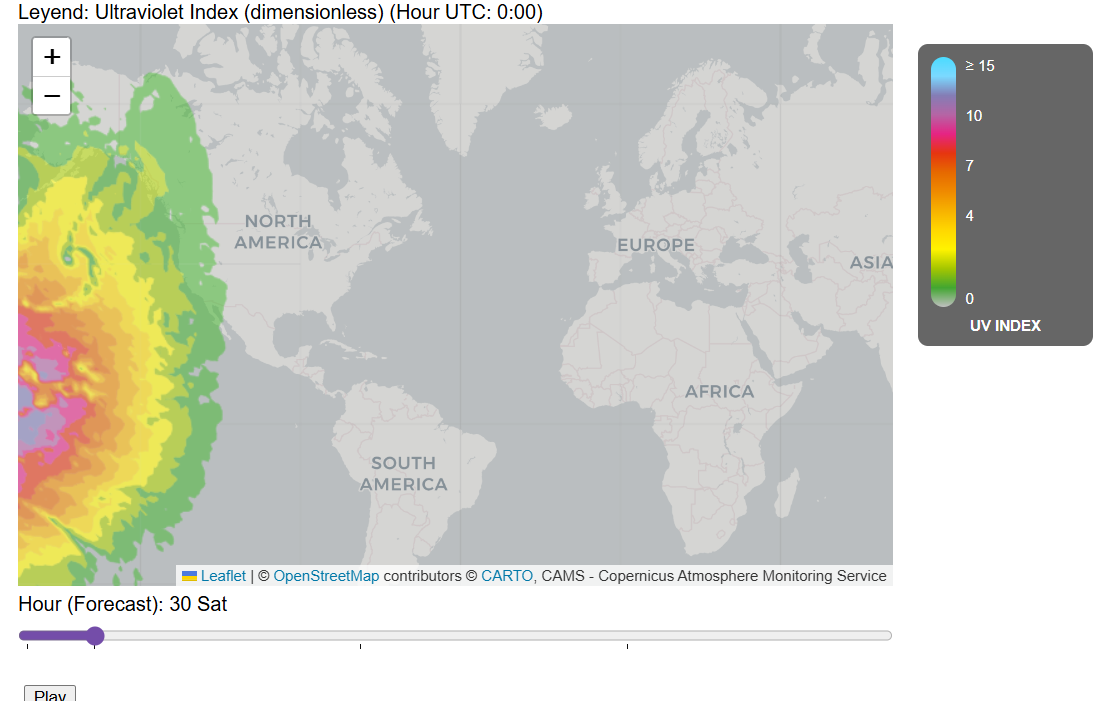
\includegraphics[width=\textwidth]{fig/animation0.png}
		\caption{Hour 0 UTC}
	\end{subfigure}
	\hfill
	\begin{subfigure}[b]{0.23\textwidth}
		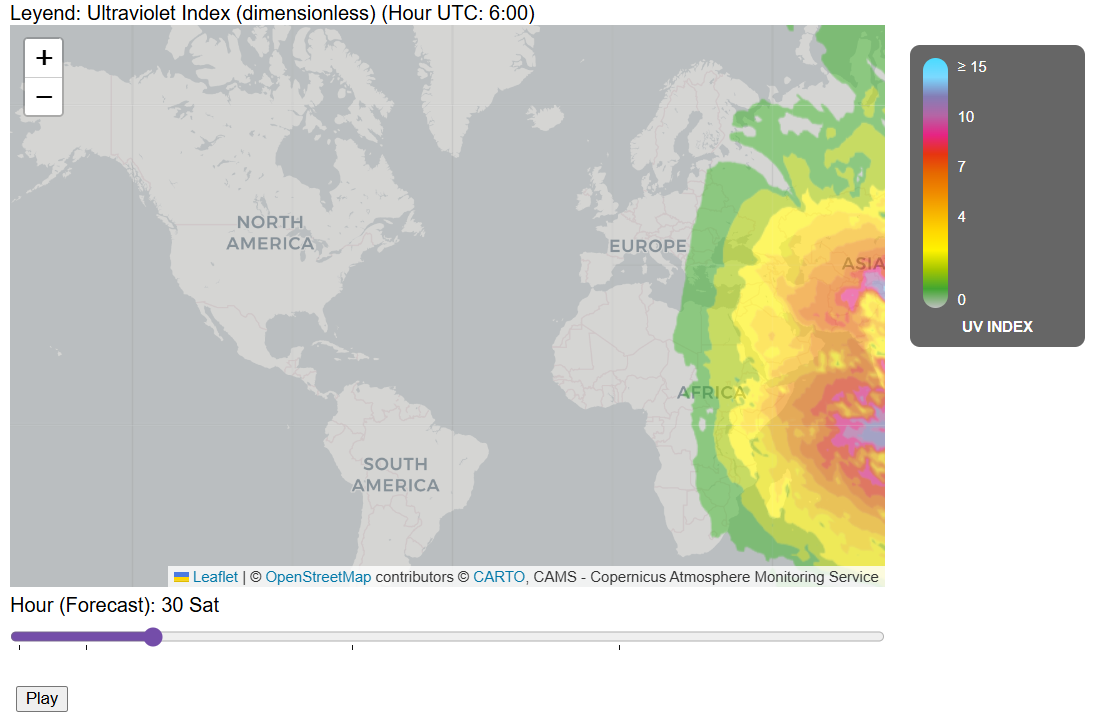
\includegraphics[width=\textwidth]{fig/animation1.png}
		\caption{Hour 6 UTC}
	\end{subfigure}
	\hfill
	\begin{subfigure}[b]{0.23\textwidth}
		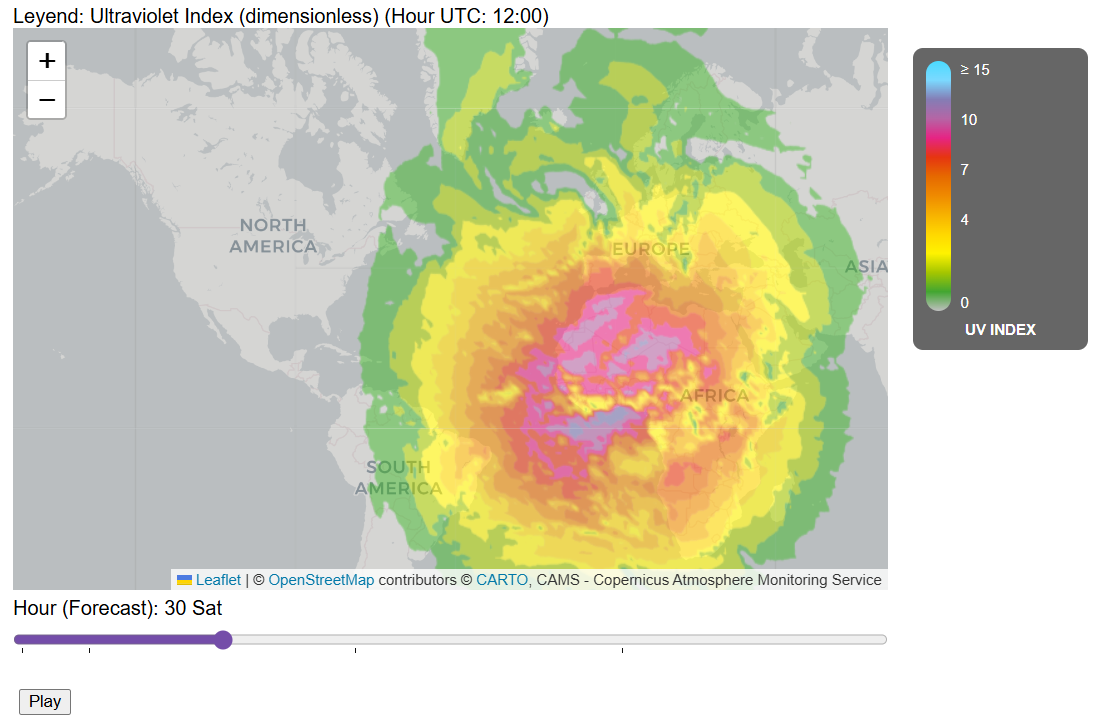
\includegraphics[width=\textwidth]{fig/animation2.png}
		\caption{Hour 12 UTC}
	\end{subfigure}
	\hfill
	\begin{subfigure}[b]{0.23\textwidth}
		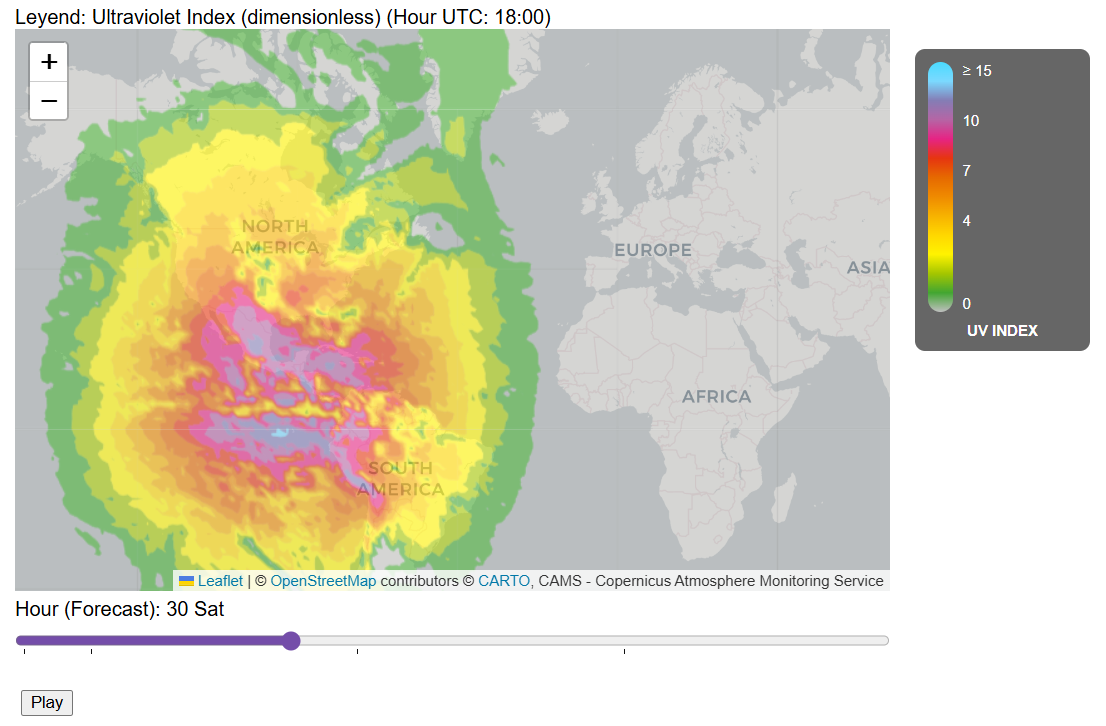
\includegraphics[width=\textwidth]{fig/animation3.png}
		\caption{Hour 18 UTC}
	\end{subfigure}
	\caption{Snapshots of the UV Index forecast animation at different forecast hours, illustrating how the pollutant layer updates as the time slider moves.}
	\label{fig:forecast-animation}
\end{figure}


\section{Summary of Results}

The web-based platform developed in this work successfully enables interactive exploration of atmospheric pollutant forecasts from CAMS. The main interface allows users to select the geographic domain and pollutant of interest, navigate through hourly forecasts, and visualize pollutant concentrations both spatially and temporally. Key features include dynamic updating of map layers, point-specific pollutant queries, interactive time-series charts, forecast animation, and data export functionality. 

The results demonstrate that the platform provides an intuitive and responsive user experience, supporting both educational and research-oriented applications. By standardizing units, integrating adaptive legends, and providing clear feedback for queries outside the forecast domain, the interface ensures consistency and transparency in data interpretation. Overall, the platform achieves its objective of making CAMS forecast data accessible and interpretable through a lightweight, browser-based solution, highlighting the potential of interactive web technologies for environmental monitoring and decision-making.

